\subsection{درک صحنه}
درک صحنه یکی از چالش‌های اساسی در زمینه بینایی ماشین است که روش‌های مختلفی برای دست‌یابی به آن ارائه شده است. با وجود تعدد پژوهش‌های موجود در این مورد، ارائه تعریف جامع و شامل برای این مفهوم کاری بسیار دشوار است. عموما این مفهوم، بسته به مورد کاربرد و هدف پژوهش، به استخراج مجموعه مشخصی از اطلاعات در مورد صحنه که برای پژوهش، کافی و مفید باشد محدود می‌شود. به همین دلیل، مجموعه اطلاعات مطلوب از تصویر که باید استخراج شود در هر پژوهش به طور خاص تعریف می‌شود.
\\
درک صحنه در زمینه تولید خودکار شرح بر تصاویر، به طور عام شامل موارد زیر می‌شود:
\begin{enumerate}
\item تشخیص اجسام موجود در صحنه و دسته‌بندی آن‌ها (مانند توپ، تلویزیون)
\item تشخیص ارتباط مکانی بین اجسام موجود در صحنه (مانند پشت، بالا)
\item دسته‌بندی محیط (مانند جنگل، دریا)
\item دسته‌بندی فعالیت به تصویر کشیده شده (مانند راه‌رفتن، خوابیدن)
\end{enumerate}

%%%%%%%%%%%%%%%%%%%%%%%%%%%%%%%%%%%%%%%%%
\subsection{روش‌های مختلف موجود}
فعالیت‌های متعددی برای تشخیص هر یک از موارد بالا انجام شده است. به طور عام می‌توان روش‌های مورد استفاده در استخراج اطلاعات مطلوب صحنه را در زمینه تولید خودکار شرح بر تصاویر به دو دسته عمده زیر تقسیم‌بندی نمود:

\begin{enumerate}
\item استفاده از مدل‌های گرافی احتمالی\enfootnote{Probabilistic Graphical Models (PGMs)} \\

در این دسته از روش‌ها، با استفاده از مدل‌های گرافی احتمالی در مورد حضور یا عدم حضور اجسام مختلف در صحنه و رابطه بین اجسام موجود استنتاج نمود. همین‌طور فرایند‌هایی مانند قطعه‌بندی تصویر\enfootnote{Image Segmentation}
در این روش‌ها با استفاده از مدل‌های گرافی احتمالی انجام می‌شوند. به عنوان نمونه، در مقاله
\cite{fidler2013sentence}
 یک مدل میدان تصادفی شرطی\enfootnote{Conditional Random Field (CRF) }
  برای تجزیه معنایی\enfootnote{Semantic Parsin
  g} تصویر ارائه شده است که با استفاده از آن می­‌توان در مورد حضور یا عدم حضور اجسام مختلف به طور توام در صحنه تصمیم­گیری کرد.
\item استفاده از شبکه‌های عصبی کانولوشنی عمیق
در این دسته از روش‌ها، با استفاده از شبکه‌های عصبی کانولوشنی عمیق، پس از قطعه‌بندی تصاویر، اقدام به تفکیک اجسام مختلف در صحنه و برچسب‌گذاری هر جسم، بسته به یادگیری انجام شده، می‌شود. به عنوان نمونه در مقاله
\cite{karpathy2015deep}
 یک شبکه عصبی کانولوشنی عمیق معرفی شده است که قادر به برچسب‌گذاری اجسام مختلف در صحنه است. برچسب‌های مورد استفاده در این پژوهش، عبارات مختلف موجود در جملات توصیف‌گر هر تصویر در مجموعه‌دادگان هستند.

\end{enumerate}

نمونه‌های متعددی از این دست پژوهش‌ها، در هر دسته، انجام شده است که در ادامه چند مورد از آن‌ها بررسی خواهد شد.

%%%%%%%%%%%%%%%%%%%%%%%%%%%%%%%%%%%%%%%%%
\subsection{روش‌های مبتنی بر مدل‌های گرافی احتمالی}

همان‌طور که قبلا ذکر شد، روش‌های مبتنی بر استفاده از مدل‌های گرافی احتمالی، از جمله پرکاربردترین روش‌ها در مرحله درک صحنه در زمینه تولید خودکار شرح بر تصاویر هستند. این روش‌ها با استفاده از نظریه گراف، آمار و احتمالات اقدام به ارائه یک توزیع احتمالی برای پارامتر مورد بررسی، با توجه به داده‌های موجود در مجموعه آموزشی می‌کنند. مدل‌های استاندارد مختلفی در پژوهش‌ها مورد استفاده قرار می‌گیرند که تعدادی از آن‌ها به عنوان نمونه در این بخش مورد بررسی قرار خواهند گرفت.
\subsubsection[استفاده از مدل میدان تصادفی مارکف]{استفاده از مدل میدان تصادفی مارکف\enfootnote{Markov Random Field (MRF)}}
مقاله
\cite{Farhadi2010every}
با استفاده از یک مدل ساده میدان تصادفی مارکف، فرایند درک صحنه را انجام می‌دهد و با استفاده از همین مدل، اقدام به تولید جملات توصیف‌گر تصویر می‌نماید. در این فصل به بررسی فرایند درک صحنه در این مقاله می‌پردازیم و بررسی فرایند تولید جمله را به فصل بعدی موکول می‌نماییم.
\\
درک صحنه در این پژوهش محدود به ارتباط بین سه مفهوم در هر تصویر شده است؛ به این معنی که به ازای هر تصویر، یک سه‌تایی «جسم، فعالیت، صحنه»\enfootnote{<Object, Activity, Scene>}
ایجاد می‌شود که بیان‌کننده اطلاعات مطلوب موجود در تصویر است. میدان\enfootnote{Field} «جسم»، دربر دارنده‌ برچسب حاصل از دسته‌بندی اجسام موجود در صحنه، میدان «فعالیت»، دربر دارنده اطلاعات مربوط به فعالیت در حال انجام و میدان «صحنه» دربردارنده اطلاعات مربوط به محیط تصویر هستند. به فضای سه‌تایی‌های ایجاد شده برای اطلاعات مطلوب در درک صحنه، فضای معنا\enfootnote{Meaning Space} می‌گویند.
\\
شکل
\ref{fig:F2010EF1}
نمایی از نگاشت اطلاعات از فضای تصاویر و جملات به فضای معنایی، نمایش می‌دهد. همان‌طور که در شکل مشخص است، به ازای هر تصویر، یک سه‌تایی معنایی ایجاد می‌شود. همین‌طور به ازای هر جمله در فضای جملات، یک سه‌تایی ایجاد می‌شود به‌طوری‌که جملات و تصاویر متناظرشان، به یک سه‌تایی یکسان، نگاشت شوند. همان‌طور که مشخص است، با داشتن نگاشت‌هایی  که خواص مذکور را داشته‌باشند، می‌توان با استفاده از سه‌تایی‌های فضای معنا، تصاویر را مدیریت کرد.

\begin{figure}[h]
\center
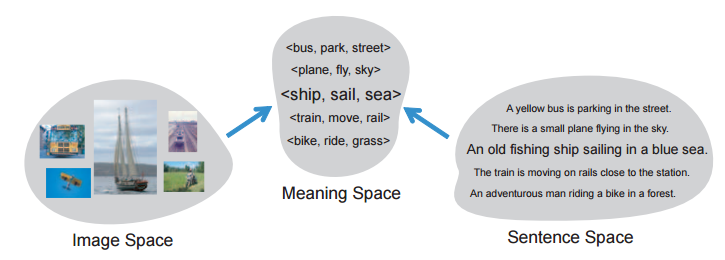
\includegraphics[scale=0.7]{./Imgs/farhadi2010every_fig1.png}
\caption{
نگاشت تصویر به فضای معنایی. فضای معنایی شامل اطلاعات مطلوب برای استخراج در فرایند درک صحنه است. به ازای هر تصویر، یک سه‌تایی ایجاد می‌شود\cite{Farhadi2010every.}
}
\label{fig:F2010EF1}
\end{figure}

مدل میدان تصادفی مارکف مورد استفاده در این پژوهش، یک مدل کوچک و ساده، شامل ۳ گره است. شکل \ref{fig:F2010EF2}
طرح‌واره‌ای از مدل میدان تصادفی مارکف مورد استفاده در این پژوهش را نمایش می‌دهد. همان‌طور که در شکل مشخص است،  به ازای هر کدام از میدان‌های تعریف شده در فضای معنایی، یک گره در این مدل وجود دارد. مقادیر مختلف در هر گره، برابر است با مقادیر مختلف موجود در میدان متناظر، در فضای معنا که با توجه به داده‌های مجموعه‌‌ ‌آموزشی مشخص می‌شوند. همین‌طور به ازای هر دو گره موجود در این مدل، یک یال بیان‌کننده ارتباط بین دو میدان در فضای معنایی وجود دارد.

\begin{figure}[h]
\center
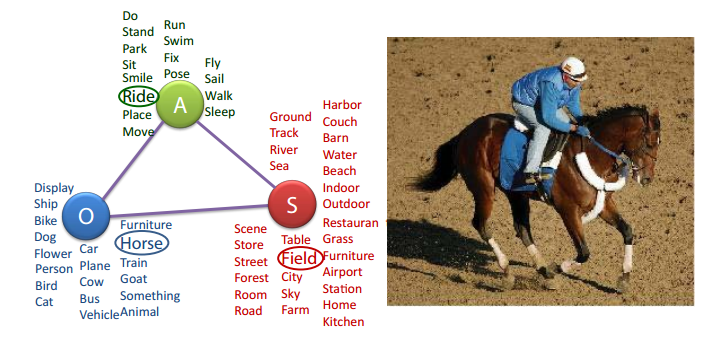
\includegraphics[scale=0.7]{./Imgs/farhadi2010every_fig2.png}
\caption{
طرح‌واره مدل میدان تصادفی مارکف ارائه شده در پژوهش \cite{Farhadi2010every} که شامل ۳ گره است. در این مدل، به ازای هر میدان از فضای معنا، یک گره وجود دارد و بین هر سه گره‌، به طور دو به دو، یک یال موجود است\cite{Farhadi2010every}.
}
\label{fig:F2010EF2}
\end{figure}

برای استنتاج در این مدل، لازم است ابتدا فاکتور‌های مورد استفاده در مدل را شناخته و مقادیر آن‌ها را مشخص نماییم. در مدل پیشنهادی، دو نوع فاکتور تعریف شده است:

\begin{enumerate}
\item فاکتور گره\\
این فاکتور، برای مشخص کردن میزان شباهت مقادیر مختلف گره با تصویر ورودی، تعریف شده‌اند. سه ویژگی‌‌های مورد استفاده برای مقداردهی این فاکتورها، شامل موارد زیر هستند:
\begin{enumerate}
	\item استفاده از آشکارکننده‌های\enfootnote{Detector} ارائه شده در مقاله \cite{felzenszwalb2008discriminatively}، 
	به منظور محاسبه امتیاز اطمینان\enfootnote{Confidence Score} برای هر دسته از اجسام موجود در مجموعه‌داده.\\
	پس از محاسبه امتیاز اطمینان همه دسته‌های موجود، دسته‌ای که بیشترین امتیاز را دارد می‌تواند به عنوان دسته‌ منتخب در میدان متناظر گره، انتخاب شود. در فرایند مقداردهی این ویژگی، قبل از انجام محاسبات، اطمینان حاصل می‌شود که از هر دسته موجود، حداقل یک تصویر در مجموعه‌داده وجود داشته باشد.
\end{enumerate}

\item فاکتور یال\\
این فاکتور، برای مشخص کردن میزان ارتباط مقادیر مختلف دو گره با یکدیگر در تصویر ورودی مورد استفاده قرار می‌گیرند.
\end{enumerate}




%%%%%%%%%%%%%%%%%%%%%%%%%%%%%%%%%%%%%%%%%
\subsection{روش‌های مبتنی بر شبکه‌های عصبی کانولوشنی عمیق}